\subsection{Greedy Heuristics Algorithm}
\todo[inline]{introductory text}

The general idea in the approach taken in this section, is using Dijkstra's algorithm for finding the shortest path with distance divided by speed as the weight of an edge. The problem then becomes, which speed must we use in the interval of $v_{min}$ and $v_{max}$. As argued previously, the optimal speed to drive can only be found by iterating over all possibilities which is a combinatorial optimization problem, and it is NP-Hard. Thus we introduce a heuristic, which promotes local optimal choices. This gives a fast path, but this might not be drivable, if there are not any charge stations on this path, thus we will need to figure out how to incorporate this.\

We will now analyse how the weight can be found, specifically the speed. The time spent passing an edge $e = (u_1, u_2)$ in the road network, is given by the following equation:
\begin{equation*}
\begin{aligned}
 & T(v,(u_1, u_2)) = \frac{D((u_1, u_2))}{v} + \frac{R_{CO}(v) * D((u_1, u_2)) - B_{cur}}{Best_{CH}(u_1)}
\end{aligned}
\end{equation*}\label{eq:drivingAndCharging}
where $v$ is the speed of the vehicle, $D(u_1, u_2)$ is the distance between vertices $u_1$ and $u_2$, $R_{CO}(v)$ is the consumption rate of the vehicle at the speed $v$, $B_{cur}$ is the current battery capacity of the vehicle and $Best_{CH}(u_1)$ is the charge rate of the best charging station previous to $u_1$ or the charge rate of $u_1$. The above equation yields a function on the form: $av^2 + bv + c$, due to the fact that $R_{CO}(v)$ is a quadratic function. $a$ , $b$ and $c$ are some constants which are given by the instance of the vehicle. 
Represented in a Cartesian coordinate system, $T(v,(u_1, u_2)))$ is a parabola, as can be seen in Figure \ref{fig:graph}. On the x-axis is the speed of the vehicle and on the y-axis is the time spent. The turning point of the graph represents the optimal speed to drive at for the given edge, denoted as $v_{opt}(e)$. The point is easily calculated by finding a tangent line with a slope of $0$. If $v_{opt}(e)$ is smaller than $v_{min}(e)$, then $v_{min}(e)$ defines the optimal speed for the edge. Similarly if $v_{opt}(e)$ is larger than $v_{max}(e)$, $v_{max}(e)$ defines the optimal speed for the edge.

\begin{figure}[!htb]
\label{fig:graph}
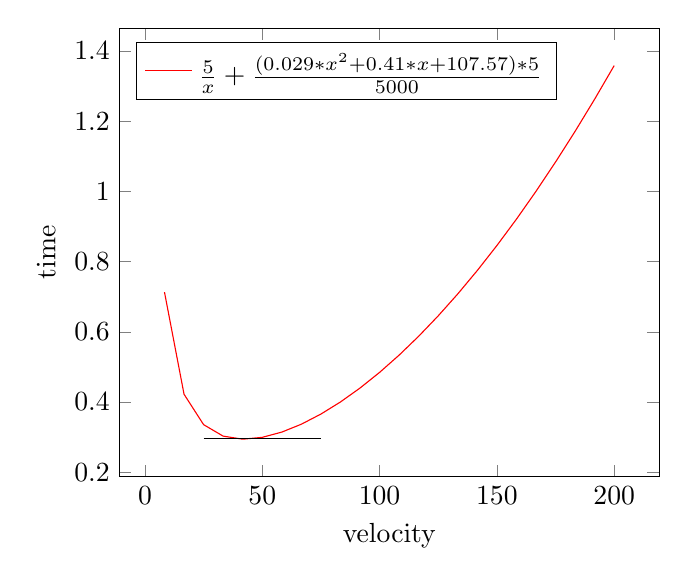
\begin{tikzpicture}
\begin{axis}[xlabel=velocity, ylabel=time,legend style={legend pos=north west}]
\addplot[draw=red,domain=0:200]{(5/x)+(((0.0286*x^2 + 0.4096*x + 107.57)*5)/5000)};
\addlegendentry{$\frac{5}{x}+\frac{(0.029*x^2 + 0.41*x + 107.57)*5}{5000}$}

\addplot[draw=black,domain=25:75]{0.295};
% \addplot[mark=*, domain=25:75] coordinates {(37,295)};
\end{axis}
\end{tikzpicture}% 
\caption{In this instance of $T(v,(u_1, u_2))$, going from $u_1$ to $u_2$, we have a distance of $5 \si{\km}$ and a charge speed of $5 \si{\kW}$ on $u_1$. The optimal speed in this case is $42.12\si{\miles\per\hour}$, which takes roughly 7 minutes to drive}
\end{figure}

The time spent driving an edge $(u_1, u_2)$, using the energy in the battery, can be found by solving:
\[B_{cur} - D(u_1, u_2) * R_{CO}(v) = 0\] 
if $v_{opt}(e)$ is lower than $v_{min}(e)$ the time used driving is set to infinity, since there is not enough energy in the battery to drive from $u_1$ to $u_2$. Otherwise $v_{opt}$ is decided in the same way when charging is considered.

\todo[inline]{more describing text}

\begin{algorithmic}
\Function{GreedyHeuristic}{$RN,s,t,EV$}
	\ForAll{$v \in RN.V$} 
		\State $v.time = \infty$
		\State $v.predecessor = NIL$
		\State $v.preCS = NIL$
		\State $v.B_{cur} = NIL$
	\EndFor
	\State $s.time = 0$
	\State $s.B_{cur} = EV.B_{cur}$

	\State $Q = PriorityQueue$
	\State $INSERT(Q, (s.time, s))$	
	\While{$Q \neq \emptyset$} 
		\State $u = extract-min(Q)$
		\ForAll{each vertex $v \in RN.adj(u)$} 
			\State $time,preCS,B_{cur},energy = travel\_time(RN, u, EV)$
			\If{$v.time > u.time + time$} 
				\State $v.time = u.time + time$
				\State $v.predecessor = u$
				\State $v.B_{cur} = B_{cur}$
				\State $v.preCS = preCS$
				\State $insert(Q, (v.time, v))$	
			\EndIf

		\EndFor
	\EndWhile
	\State \Return $t.time, t.path$
\EndFunction
\end{algorithmic}\label{alg:fastest_path}
